\subsection{Measuring \texorpdfstring{$T_1$}{T1} for Water, Alcohol and Rubber Using the Inversion Recovery Sequence} \label{B4}

\begin{comment}
\begin{itemize}
\item Write at the beginning of this section what the inversion recovery sequence is and how we are using it to measure $T_1$ \textbf{(5 mins)}
\item It says to use a repetition time at least 5*$T_1$. Why do we do that? How does it impact our data? Discuss here \textbf{(5 min)}
\item Show how you found the initial magnetization data points for one of the samples ****this involves probably shifting the graphs up so that they approach 0****  (show a plot with a labeled data point) \textbf{(10 min)}
\item write up a sample uncertainty calculation for getting one of the values (the uncertainty is the uncertainty associated from reading off the graph + noise), include that calculation in the report. There will be an uncertainty associated with both the time and magnetization values \textbf{(10 mins)}
\item get each value for the initial magnetization and the time for each trial for every sample, record the uncertainties if they differ between different samples because of a difference in scale \textbf{(30 mins)}
\item plot the values obtained for each of the samples, include a graph with error bars (the uncertainties from above), there should be horiziontial and vertical bars because we're approximating both the time and voltage. given units and a title. \textbf{(15 mins)}
\item write up the rearrangement of the $T_1$ equation where you take a the ln and plot the corresponding relationship for each sample \textbf{(30 mins)}. 
\item Use a linear regression (specify which program and function you used) to find $T_1$ for each of the samples. Put in the coefficients with uncertainties that your linear regression outputted. \textbf{(15 mins)}
\item Show a sample calculation for calculating $T_1$ using the equation. Include sample uncertainity calculation. \textbf{(10 mins)}
\item Write up what the zero-crossing method is. \textbf{(5 mins)}.
\item Calculate $T_1$ and its uncertainty for each using the zero-crossing method. Show sample uncertainty calculation. \textbf{(30 mins)}
\item Compare the $T_1$ from inversion to zero crossing using the \% difference for each sample. Show a sample calculation. \textbf{(15 mins)}
\item Talk about why the $T_1$'s are different for each of the samples and the physics. 
\end{itemize}
\end{comment}

An inversion recovery (IR) protocol was performed on the three samples using a 180-$\tau$-90 pulse sequence and all parameters set to maximize the signal. This method is called inversion recovery as the magnetization is initially \textit{inverted} to the negative $z$-direction. As it \textit{recovers} to the positive $z$-direction, the second 90$\degree$ pulse knocks whatever total magnetization is in the $z$ direction to the $xy$-plane -- essentially probing what amount the magnetization has recovered in the time $\tau$.\\

The magnetization at the time-delay of $\tau$ is given by equation \ref{eqn:IR},
\begin{align*}
    M_z(\tau) &= M_0(1-2e^{-\tau/T_1} )\\
    \intertext{Rearranging and taking the natural logarithm of both sides,}
     -\frac{\tau}{T_1} &= \ln \left( \frac{1}{2} -\frac{M_z(\tau)}{2M_0} \right) \numberthis\label{eqn:B4:lnfit}
\end{align*}

Each data trace was zero-shifted and filtered using a Gaussian filter (discussed in Appendix \ref{append:process}), followed by a simple peak detection to determine the time-delay $\tau$ and the peak magnetization $M_z(\tau)$ (see Figure \ref{fig:B4:timetraces}). The initial magnetization, $M_0$, was recorded as the maximum of a single FID for each sample (see, for example, Figure \ref{fig:B1:pulses}). These values were extracted from each experiment and compiled in Figure \ref{fig:B4:expfit}. Using Equation \ref{eqn:B4:lnfit} to fit the data to linear slope we calculate $T_1$ for each sample, which are tabulated in Table \ref{tab:B4:T1vals}. \\

The $T_1$ values for each sample can also be calculated using the zero-crossing (ZC) method. From Equation \ref{eqn:B4:lnfit} with $M_z(t) = 0$,
\begin{align*}
    T_1 &= \frac{\tau}{\ln(2)} \numberthis
\end{align*}

So, using the above equation with a rough estimate of the value for $\tau$ where $M_z(\tau)=0$ we can generate a rough guess of $T_1$.

\begin{figure}[H]
    \centering
    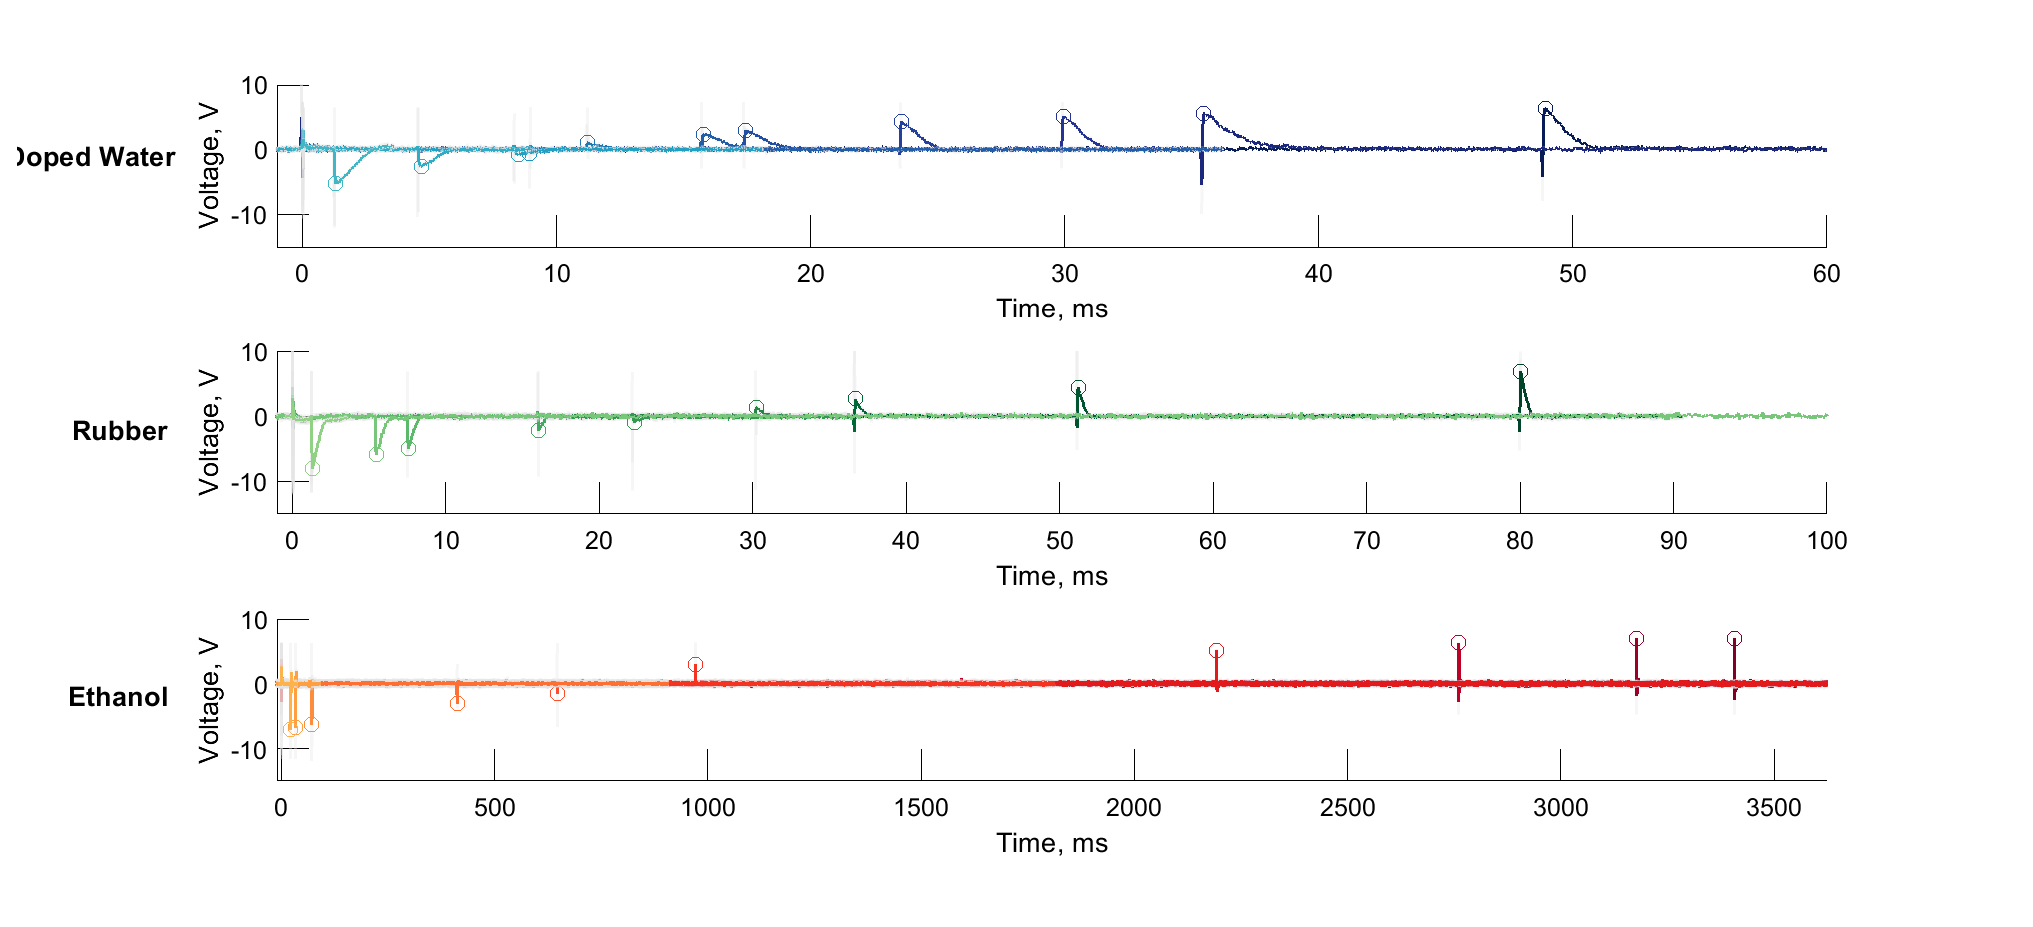
\includegraphics[width=\textwidth]{figures/B4/B4_1.eps}
    \caption{Oscilloscope traces of IR sequence for three samples after zero-shifting and filtering to determine peak magnetization values for each value of $\tau$. Solid lines are the filtered data, light gray lines represent the raw, unfiltered data, and circles represent the computed peak magnetization values at $\tau$.}
    \label{fig:B4:timetraces}
\end{figure}

\begin{figure}[H]
    \centering
    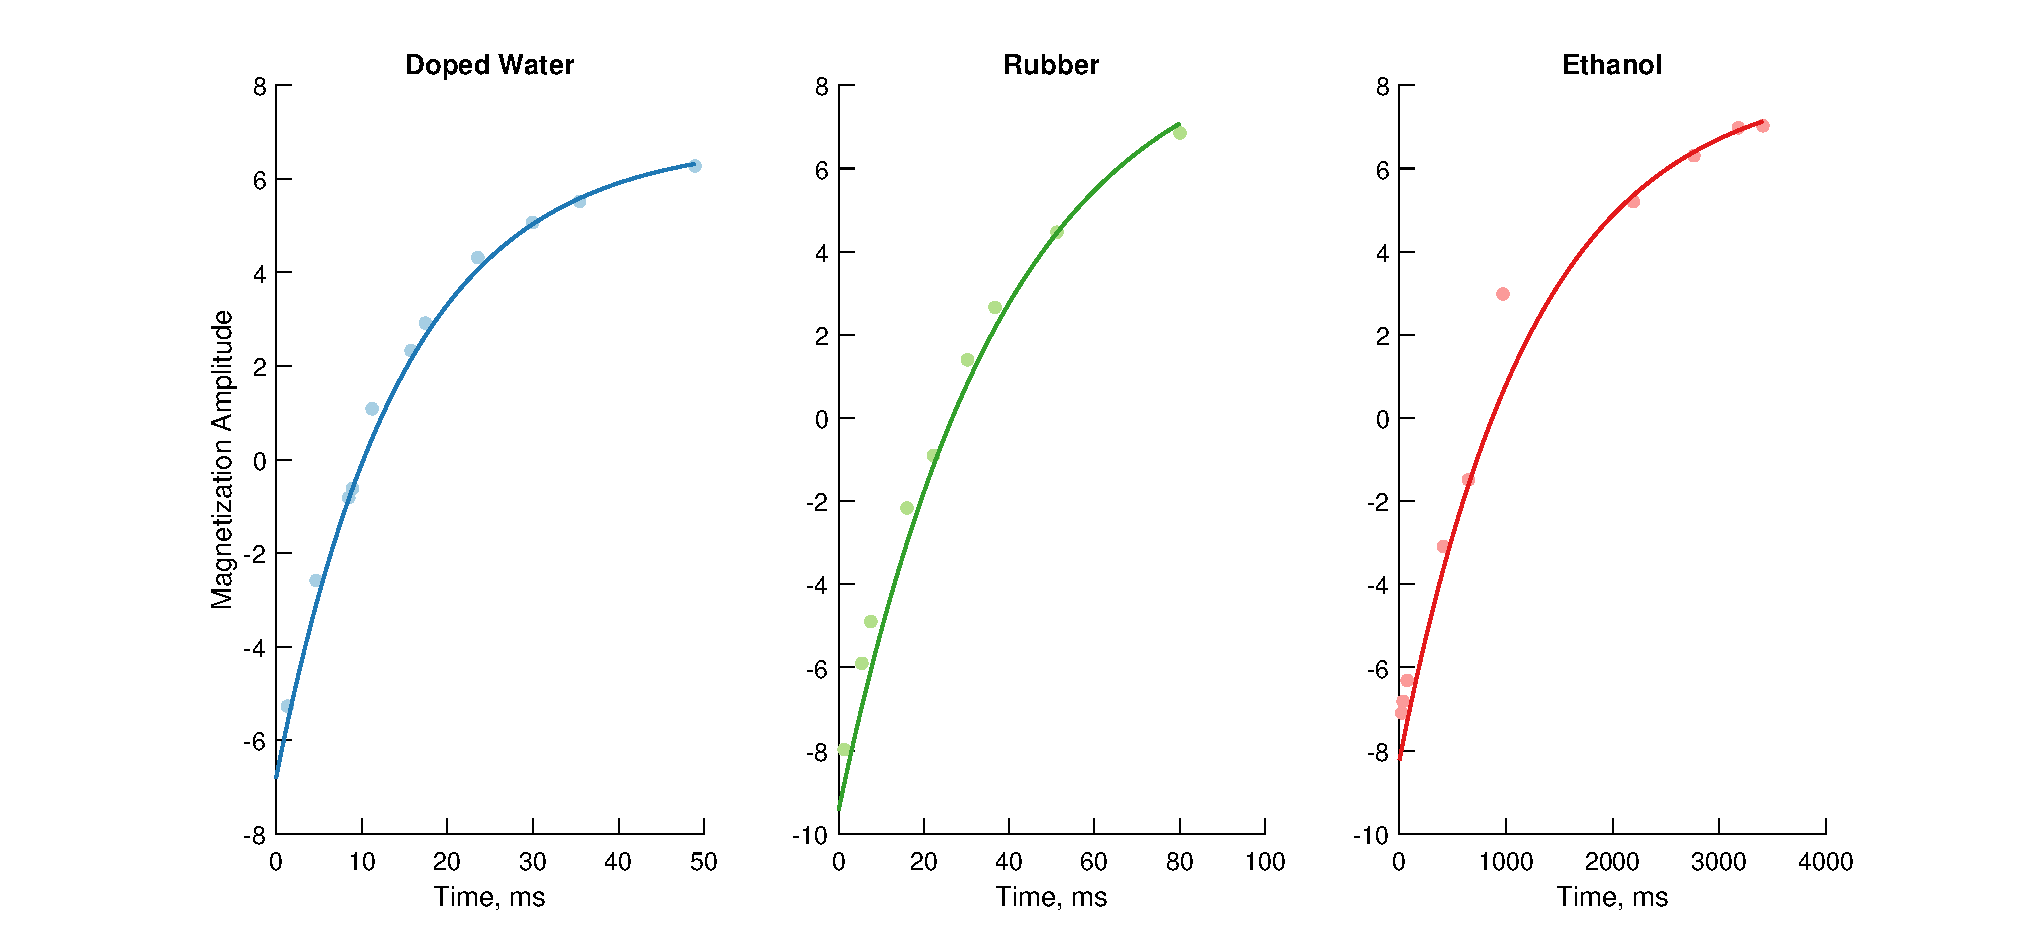
\includegraphics[width=\textwidth]{figures/B4/B4_2.eps}
    \caption{Peak magnetization values at a time-delay of $\tau$ (coloured circles) with the corresponding fit (solid line), calculated from the traces demonstrated in Figure \ref{fig:B4:timetraces} for doped water, ethanol and rubber.}
    \label{fig:B4:expfit}
\end{figure}

\begin{table}[H]
    \centering
    \begin{tabular}{c|c|c|c}
    \toprule
    \textbf{Sample} & IR Method $T_1$ (ms) & ZC Method $T_1$ (ms) & Percent Difference (\%)\\ \midrule
        Doped Water &  $14.74 \pm 0.41$ & $14.0\pm1.2$ & 5.15 \\
        Ethanol &  $1257 \pm 82$ & $1117\pm168$ & 11.79 \\
        Rubber &  $38.48 \pm 2.09$ & $37.2\pm 3.1$ & 3.38 \\ \bottomrule
    \end{tabular}
    \caption{$T_1$ values for three samples calculated using the inversion-recovery (IR) sequence (fit parameters from Figure \ref{fig:B4:expfit}), the zero-crossing (ZC) method, and the percent difference between the two methods.}
    \label{tab:B4:T1vals}
\end{table}

The uncertainty range of the ZC method always encloses the value calculated from the IR value, as the uncertainty in the ZC method is highly inaccurate. However this does not hold true vice versa, as the uncertainty in the IR measurements is much lesser and does not encompass the ZC method values. For ethanol, as the time scales are much longer, it is difficult to generate an accurate estimation of where the zero-crossing point is -- which is reflected in the percent difference from our more accurate IR method. The ZC method is a suitable procedure for estimating the $T_1$ constant, but as it is based off a single point, is not suitable for as a true measurement.\\ 

We may also compare this method to that used in Section \ref{B3}. Comparing the values of $T_1$ using the IR method (Table \ref{tab:B4:T1vals}) and the SR method (Table \ref{tab:B3:T1values}), the percent differences are $9.91\%$ for doped water, $19.94\%$ for ethanol, and $11.84\%$ for rubber. While both the IR and SR methods have limitations and errors, the IR method is more accurate for calculating $T_1$ -- as generating a fit over many data points reduces the propagation of random errors, which does not happen in Section \ref{B3} with the SR method. Thus, $T_1$ values calculated using the IR method, tabulated in Table \ref{tab:B4:T1vals}, are considered as our most realistic time constants. \\